\PassOptionsToPackage{unicode=true}{hyperref} % options for packages loaded elsewhere
\PassOptionsToPackage{hyphens}{url}
%
\documentclass[
]{article}
\usepackage{lmodern}
\usepackage{amssymb,amsmath}
\usepackage{ifxetex,ifluatex}
\ifnum 0\ifxetex 1\fi\ifluatex 1\fi=0 % if pdftex
  \usepackage[T1]{fontenc}
  \usepackage[utf8]{inputenc}
  \usepackage{textcomp} % provides euro and other symbols
\else % if luatex or xelatex
  \usepackage{unicode-math}
  \defaultfontfeatures{Scale=MatchLowercase}
  \defaultfontfeatures[\rmfamily]{Ligatures=TeX,Scale=1}
\fi
% use upquote if available, for straight quotes in verbatim environments
\IfFileExists{upquote.sty}{\usepackage{upquote}}{}
\IfFileExists{microtype.sty}{% use microtype if available
  \usepackage[]{microtype}
  \UseMicrotypeSet[protrusion]{basicmath} % disable protrusion for tt fonts
}{}
\makeatletter
\@ifundefined{KOMAClassName}{% if non-KOMA class
  \IfFileExists{parskip.sty}{%
    \usepackage{parskip}
  }{% else
    \setlength{\parindent}{0pt}
    \setlength{\parskip}{6pt plus 2pt minus 1pt}}
}{% if KOMA class
  \KOMAoptions{parskip=half}}
\makeatother
\usepackage{xcolor}
\IfFileExists{xurl.sty}{\usepackage{xurl}}{} % add URL line breaks if available
\IfFileExists{bookmark.sty}{\usepackage{bookmark}}{\usepackage{hyperref}}
\hypersetup{
  pdftitle={Introduction to R Basics},
  pdfborder={0 0 0},
  breaklinks=true}
\urlstyle{same}  % don't use monospace font for urls
\usepackage[margin=1in]{geometry}
\usepackage{color}
\usepackage{fancyvrb}
\newcommand{\VerbBar}{|}
\newcommand{\VERB}{\Verb[commandchars=\\\{\}]}
\DefineVerbatimEnvironment{Highlighting}{Verbatim}{commandchars=\\\{\}}
% Add ',fontsize=\small' for more characters per line
\usepackage{framed}
\definecolor{shadecolor}{RGB}{248,248,248}
\newenvironment{Shaded}{\begin{snugshade}}{\end{snugshade}}
\newcommand{\AlertTok}[1]{\textcolor[rgb]{0.94,0.16,0.16}{#1}}
\newcommand{\AnnotationTok}[1]{\textcolor[rgb]{0.56,0.35,0.01}{\textbf{\textit{#1}}}}
\newcommand{\AttributeTok}[1]{\textcolor[rgb]{0.77,0.63,0.00}{#1}}
\newcommand{\BaseNTok}[1]{\textcolor[rgb]{0.00,0.00,0.81}{#1}}
\newcommand{\BuiltInTok}[1]{#1}
\newcommand{\CharTok}[1]{\textcolor[rgb]{0.31,0.60,0.02}{#1}}
\newcommand{\CommentTok}[1]{\textcolor[rgb]{0.56,0.35,0.01}{\textit{#1}}}
\newcommand{\CommentVarTok}[1]{\textcolor[rgb]{0.56,0.35,0.01}{\textbf{\textit{#1}}}}
\newcommand{\ConstantTok}[1]{\textcolor[rgb]{0.00,0.00,0.00}{#1}}
\newcommand{\ControlFlowTok}[1]{\textcolor[rgb]{0.13,0.29,0.53}{\textbf{#1}}}
\newcommand{\DataTypeTok}[1]{\textcolor[rgb]{0.13,0.29,0.53}{#1}}
\newcommand{\DecValTok}[1]{\textcolor[rgb]{0.00,0.00,0.81}{#1}}
\newcommand{\DocumentationTok}[1]{\textcolor[rgb]{0.56,0.35,0.01}{\textbf{\textit{#1}}}}
\newcommand{\ErrorTok}[1]{\textcolor[rgb]{0.64,0.00,0.00}{\textbf{#1}}}
\newcommand{\ExtensionTok}[1]{#1}
\newcommand{\FloatTok}[1]{\textcolor[rgb]{0.00,0.00,0.81}{#1}}
\newcommand{\FunctionTok}[1]{\textcolor[rgb]{0.00,0.00,0.00}{#1}}
\newcommand{\ImportTok}[1]{#1}
\newcommand{\InformationTok}[1]{\textcolor[rgb]{0.56,0.35,0.01}{\textbf{\textit{#1}}}}
\newcommand{\KeywordTok}[1]{\textcolor[rgb]{0.13,0.29,0.53}{\textbf{#1}}}
\newcommand{\NormalTok}[1]{#1}
\newcommand{\OperatorTok}[1]{\textcolor[rgb]{0.81,0.36,0.00}{\textbf{#1}}}
\newcommand{\OtherTok}[1]{\textcolor[rgb]{0.56,0.35,0.01}{#1}}
\newcommand{\PreprocessorTok}[1]{\textcolor[rgb]{0.56,0.35,0.01}{\textit{#1}}}
\newcommand{\RegionMarkerTok}[1]{#1}
\newcommand{\SpecialCharTok}[1]{\textcolor[rgb]{0.00,0.00,0.00}{#1}}
\newcommand{\SpecialStringTok}[1]{\textcolor[rgb]{0.31,0.60,0.02}{#1}}
\newcommand{\StringTok}[1]{\textcolor[rgb]{0.31,0.60,0.02}{#1}}
\newcommand{\VariableTok}[1]{\textcolor[rgb]{0.00,0.00,0.00}{#1}}
\newcommand{\VerbatimStringTok}[1]{\textcolor[rgb]{0.31,0.60,0.02}{#1}}
\newcommand{\WarningTok}[1]{\textcolor[rgb]{0.56,0.35,0.01}{\textbf{\textit{#1}}}}
\usepackage{graphicx,grffile}
\makeatletter
\def\maxwidth{\ifdim\Gin@nat@width>\linewidth\linewidth\else\Gin@nat@width\fi}
\def\maxheight{\ifdim\Gin@nat@height>\textheight\textheight\else\Gin@nat@height\fi}
\makeatother
% Scale images if necessary, so that they will not overflow the page
% margins by default, and it is still possible to overwrite the defaults
% using explicit options in \includegraphics[width, height, ...]{}
\setkeys{Gin}{width=\maxwidth,height=\maxheight,keepaspectratio}
\setlength{\emergencystretch}{3em}  % prevent overfull lines
\providecommand{\tightlist}{%
  \setlength{\itemsep}{0pt}\setlength{\parskip}{0pt}}
\setcounter{secnumdepth}{-2}
% Redefines (sub)paragraphs to behave more like sections
\ifx\paragraph\undefined\else
  \let\oldparagraph\paragraph
  \renewcommand{\paragraph}[1]{\oldparagraph{#1}\mbox{}}
\fi
\ifx\subparagraph\undefined\else
  \let\oldsubparagraph\subparagraph
  \renewcommand{\subparagraph}[1]{\oldsubparagraph{#1}\mbox{}}
\fi

% set default figure placement to htbp
\makeatletter
\def\fps@figure{htbp}
\makeatother


\title{Introduction to R Basics}
\author{}
\date{\vspace{-2.5em}}

\begin{document}
\maketitle

\hypertarget{overview}{%
\section{Overview}\label{overview}}

\#\#This R Markdown file covers the basics of R programming, how to set
up environments, explore data types, and execute basic functions with
illustrative examples using popular R packages.

\hypertarget{installation-and-setup}{%
\subsection{Installation and Setup}\label{installation-and-setup}}

\begin{Shaded}
\begin{Highlighting}[]
\CommentTok{# Install required packages}
\ControlFlowTok{if}\NormalTok{ (}\OperatorTok{!}\KeywordTok{requireNamespace}\NormalTok{(}\StringTok{"tidyverse"}\NormalTok{, }\DataTypeTok{quietly =} \OtherTok{TRUE}\NormalTok{)) }\KeywordTok{install.packages}\NormalTok{(}\StringTok{"tidyverse"}\NormalTok{)}
\ControlFlowTok{if}\NormalTok{ (}\OperatorTok{!}\KeywordTok{requireNamespace}\NormalTok{(}\StringTok{"ggplot2"}\NormalTok{, }\DataTypeTok{quietly =} \OtherTok{TRUE}\NormalTok{)) }\KeywordTok{install.packages}\NormalTok{(}\StringTok{"ggplot2"}\NormalTok{)}
\ControlFlowTok{if}\NormalTok{ (}\OperatorTok{!}\KeywordTok{requireNamespace}\NormalTok{(}\StringTok{"dplyr"}\NormalTok{, }\DataTypeTok{quietly =} \OtherTok{TRUE}\NormalTok{)) }\KeywordTok{install.packages}\NormalTok{(}\StringTok{"dplyr"}\NormalTok{) }
\end{Highlighting}
\end{Shaded}

\hypertarget{r-basic-data-structures}{%
\subsection{R Basic Data structures}\label{r-basic-data-structures}}

\begin{Shaded}
\begin{Highlighting}[]
\CommentTok{# Scalars, vectors, lists, and data frames}
\NormalTok{scalar <-}\StringTok{ }\DecValTok{42}
\NormalTok{vector <-}\StringTok{ }\KeywordTok{c}\NormalTok{(}\DecValTok{1}\NormalTok{, }\DecValTok{2}\NormalTok{, }\DecValTok{3}\NormalTok{, }\DecValTok{4}\NormalTok{, }\DecValTok{5}\NormalTok{)}
\NormalTok{list_example <-}\StringTok{ }\KeywordTok{list}\NormalTok{(}\DataTypeTok{name =} \StringTok{"R"}\NormalTok{, }\DataTypeTok{version =} \FloatTok{4.0}\NormalTok{, }\DataTypeTok{features =} \KeywordTok{c}\NormalTok{(}\StringTok{"data"}\NormalTok{, }\StringTok{"graphics"}\NormalTok{))}
\NormalTok{data_frame_example <-}\StringTok{ }\KeywordTok{data.frame}\NormalTok{(}\DataTypeTok{ID =} \DecValTok{1}\OperatorTok{:}\DecValTok{3}\NormalTok{, }\DataTypeTok{Value =} \KeywordTok{c}\NormalTok{(}\DecValTok{10}\NormalTok{, }\DecValTok{20}\NormalTok{, }\DecValTok{30}\NormalTok{))}

\CommentTok{# Output types}
\KeywordTok{class}\NormalTok{(scalar)}
\end{Highlighting}
\end{Shaded}

\begin{verbatim}
## [1] "numeric"
\end{verbatim}

\begin{Shaded}
\begin{Highlighting}[]
\KeywordTok{class}\NormalTok{(vector)}
\end{Highlighting}
\end{Shaded}

\begin{verbatim}
## [1] "numeric"
\end{verbatim}

\begin{Shaded}
\begin{Highlighting}[]
\KeywordTok{class}\NormalTok{(list_example)}
\end{Highlighting}
\end{Shaded}

\begin{verbatim}
## [1] "list"
\end{verbatim}

\begin{Shaded}
\begin{Highlighting}[]
\KeywordTok{class}\NormalTok{(data_frame_example)}
\end{Highlighting}
\end{Shaded}

\begin{verbatim}
## [1] "data.frame"
\end{verbatim}

\hypertarget{basic-arithmetic}{%
\subsection{Basic arithmetic}\label{basic-arithmetic}}

\hypertarget{in-its-most-basic-form-r-can-be-used-as-a-simple-calculator.-consider-the-following-arithmetic-operators}{%
\paragraph{In its most basic form, R can be used as a simple calculator.
Consider the following arithmetic
operators:}\label{in-its-most-basic-form-r-can-be-used-as-a-simple-calculator.-consider-the-following-arithmetic-operators}}

\hypertarget{addition}{%
\paragraph{\texorpdfstring{\textbf{Addition}:
\texttt{+}}{Addition: +}}\label{addition}}

\hypertarget{subtraction--}{%
\paragraph{\texorpdfstring{\textbf{Subtraction}:
\texttt{-}}{Subtraction: -}}\label{subtraction--}}

\hypertarget{multiplication}{%
\paragraph{\texorpdfstring{\textbf{Multiplication}:
\texttt{*}}{Multiplication: *}}\label{multiplication}}

\hypertarget{division}{%
\paragraph{\texorpdfstring{\textbf{Division}:
\texttt{/}}{Division: /}}\label{division}}

\hypertarget{exponentiation}{%
\paragraph{\texorpdfstring{\textbf{Exponentiation}:
\texttt{\^{}}}{Exponentiation: \^{}}}\label{exponentiation}}

\hypertarget{modulo}{%
\paragraph{\texorpdfstring{\textbf{Modulo}:
\texttt{\%\%}}{Modulo: \%\%}}\label{modulo}}

\begin{Shaded}
\begin{Highlighting}[]
\NormalTok{addition <-}\StringTok{ }\DecValTok{7} \OperatorTok{+}\StringTok{ }\DecValTok{3}
\NormalTok{subtraction <-}\StringTok{ }\DecValTok{7} \OperatorTok{-}\StringTok{ }\DecValTok{3}
\NormalTok{multiplication <-}\StringTok{ }\DecValTok{7} \OperatorTok{*}\StringTok{ }\DecValTok{3}
\NormalTok{division <-}\StringTok{ }\DecValTok{7} \OperatorTok{/}\StringTok{ }\DecValTok{3}
\end{Highlighting}
\end{Shaded}

\hypertarget{plots}{%
\subsection{Plots}\label{plots}}

\begin{Shaded}
\begin{Highlighting}[]
\KeywordTok{library}\NormalTok{(ggplot2)}
\end{Highlighting}
\end{Shaded}

\begin{verbatim}
## Warning: package 'ggplot2' was built under R version 4.2.3
\end{verbatim}

\begin{Shaded}
\begin{Highlighting}[]
\CommentTok{# Example dataset}
\NormalTok{data <-}\StringTok{ }\KeywordTok{data.frame}\NormalTok{(}\DataTypeTok{x =}\NormalTok{ (}\DecValTok{1}\OperatorTok{:}\DecValTok{10}\NormalTok{)}\OperatorTok{^}\DecValTok{3}\NormalTok{, }\DataTypeTok{y =}\NormalTok{ (}\DecValTok{1}\OperatorTok{:}\DecValTok{10}\NormalTok{)}\OperatorTok{^}\DecValTok{3}\NormalTok{)}
\CommentTok{#With the plot() funtion}
\CommentTok{#To change the type of plot can just need to change the letter in the type="x" with p as point and l as lines}
\CommentTok{#Scatter plot}
\KeywordTok{plot}\NormalTok{(data}\OperatorTok{$}\NormalTok{x,data}\OperatorTok{$}\NormalTok{y,}\DataTypeTok{type=}\StringTok{"p"}\NormalTok{)}
\end{Highlighting}
\end{Shaded}

\includegraphics{Basics_R_files/figure-latex/unnamed-chunk-3-1.pdf}

\begin{Shaded}
\begin{Highlighting}[]
\CommentTok{##Line plot }
\KeywordTok{plot}\NormalTok{(data}\OperatorTok{$}\NormalTok{x,data}\OperatorTok{$}\NormalTok{y,}\DataTypeTok{type=}\StringTok{"l"}\NormalTok{)}
\end{Highlighting}
\end{Shaded}

\includegraphics{Basics_R_files/figure-latex/unnamed-chunk-3-2.pdf}

\begin{Shaded}
\begin{Highlighting}[]
\CommentTok{##Both}
\KeywordTok{plot}\NormalTok{(data}\OperatorTok{$}\NormalTok{x,data}\OperatorTok{$}\NormalTok{y,}\DataTypeTok{type=}\StringTok{"b"}\NormalTok{,}\DataTypeTok{col=}\StringTok{"blue"}\NormalTok{)}
\end{Highlighting}
\end{Shaded}

\includegraphics{Basics_R_files/figure-latex/unnamed-chunk-3-3.pdf}

\begin{Shaded}
\begin{Highlighting}[]
\CommentTok{##We can also stack the plots together}
\KeywordTok{plot}\NormalTok{(data}\OperatorTok{$}\NormalTok{x,data}\OperatorTok{$}\NormalTok{y,}\DataTypeTok{type=}\StringTok{"p"}\NormalTok{)}
\KeywordTok{lines}\NormalTok{(data}\OperatorTok{$}\NormalTok{x,data}\OperatorTok{$}\NormalTok{y)}
\end{Highlighting}
\end{Shaded}

\includegraphics{Basics_R_files/figure-latex/unnamed-chunk-3-4.pdf}

\begin{Shaded}
\begin{Highlighting}[]
\CommentTok{# Scatter plot}
\KeywordTok{library}\NormalTok{(ggplot2)}

\KeywordTok{ggplot}\NormalTok{(data, }\KeywordTok{aes}\NormalTok{(}\DataTypeTok{x =}\NormalTok{ x, }\DataTypeTok{y =}\NormalTok{ y)) }\OperatorTok{+}
\StringTok{  }\KeywordTok{geom_point}\NormalTok{() }\OperatorTok{+}
\StringTok{  }\KeywordTok{ggtitle}\NormalTok{(}\StringTok{"Scatter Plot of x and y^2"}\NormalTok{)}
\end{Highlighting}
\end{Shaded}

\includegraphics{Basics_R_files/figure-latex/unnamed-chunk-3-5.pdf}

\begin{Shaded}
\begin{Highlighting}[]
\KeywordTok{library}\NormalTok{(ggplot2)}

\CommentTok{# Example dataset}
\NormalTok{data <-}\StringTok{ }\KeywordTok{data.frame}\NormalTok{(}\DataTypeTok{x =} \DecValTok{1}\OperatorTok{:}\DecValTok{10}\NormalTok{, }\DataTypeTok{y =}\NormalTok{ (}\DecValTok{1}\OperatorTok{:}\DecValTok{10}\NormalTok{)}\OperatorTok{^}\DecValTok{2}\NormalTok{)}

\CommentTok{# Scatter plot}
\KeywordTok{ggplot}\NormalTok{(data, }\KeywordTok{aes}\NormalTok{(}\DataTypeTok{x =}\NormalTok{ x, }\DataTypeTok{y =}\NormalTok{ y)) }\OperatorTok{+}
\StringTok{  }\KeywordTok{geom_point}\NormalTok{() }\OperatorTok{+}
\StringTok{  }\KeywordTok{ggtitle}\NormalTok{(}\StringTok{"Scatter Plot of x and y^2"}\NormalTok{)}
\end{Highlighting}
\end{Shaded}

\includegraphics{Basics_R_files/figure-latex/unnamed-chunk-4-1.pdf}

\hypertarget{the-same-way-we-used-the-operators-as-a-calculator-we-can-use-them-to-perform-operations-on-vectors-and-matrices.}{%
\subsubsection{The same way we used the operators as a calculator, we
can use them to perform operations on vectors and
matrices.}\label{the-same-way-we-used-the-operators-as-a-calculator-we-can-use-them-to-perform-operations-on-vectors-and-matrices.}}

\begin{Shaded}
\begin{Highlighting}[]
\CommentTok{## Vector Arithmetic with Visualization}
\CommentTok{# Creating vectors}
\NormalTok{vector_a <-}\StringTok{ }\KeywordTok{c}\NormalTok{(}\DecValTok{1}\NormalTok{, }\DecValTok{2}\NormalTok{, }\DecValTok{3}\NormalTok{, }\DecValTok{4}\NormalTok{, }\DecValTok{5}\NormalTok{)}
\NormalTok{vector_b <-}\StringTok{ }\KeywordTok{c}\NormalTok{(}\DecValTok{10}\NormalTok{, }\DecValTok{20}\NormalTok{, }\DecValTok{30}\NormalTok{, }\DecValTok{40}\NormalTok{, }\DecValTok{50}\NormalTok{)}

\CommentTok{# Element-wise operations}
\NormalTok{vector_sum <-}\StringTok{ }\NormalTok{vector_a }\OperatorTok{+}\StringTok{ }\NormalTok{vector_b}
\NormalTok{vector_diff <-}\StringTok{ }\NormalTok{vector_b }\OperatorTok{-}\StringTok{ }\NormalTok{vector_a}
\NormalTok{vector_prod <-}\StringTok{ }\NormalTok{vector_a }\OperatorTok{*}\StringTok{ }\NormalTok{vector_b}
\NormalTok{vector_div <-}\StringTok{ }\NormalTok{vector_b }\OperatorTok{/}\StringTok{ }\NormalTok{vector_a}

\CommentTok{# Scalar operations}
\NormalTok{vector_scaled <-}\StringTok{ }\NormalTok{vector_a }\OperatorTok{*}\StringTok{ }\DecValTok{2}

\CommentTok{# Combine results into a data frame for visualization}
\NormalTok{vector_results <-}\StringTok{ }\KeywordTok{data.frame}\NormalTok{(}
  \DataTypeTok{Index =} \DecValTok{1}\OperatorTok{:}\KeywordTok{length}\NormalTok{(vector_a),}
  \DataTypeTok{VectorA =}\NormalTok{ vector_a,}
  \DataTypeTok{VectorB =}\NormalTok{ vector_b,}
  \DataTypeTok{Sum =}\NormalTok{ vector_sum,}
  \DataTypeTok{Difference =}\NormalTok{ vector_diff,}
  \DataTypeTok{Product =}\NormalTok{ vector_prod,}
  \DataTypeTok{Division =}\NormalTok{ vector_div,}
  \DataTypeTok{Scaled =}\NormalTok{ vector_scaled}
\NormalTok{)}

\NormalTok{vector_results}
\end{Highlighting}
\end{Shaded}

\begin{verbatim}
##   Index VectorA VectorB Sum Difference Product Division Scaled
## 1     1       1      10  11          9      10       10      2
## 2     2       2      20  22         18      40       10      4
## 3     3       3      30  33         27      90       10      6
## 4     4       4      40  44         36     160       10      8
## 5     5       5      50  55         45     250       10     10
\end{verbatim}

\hypertarget{tables}{%
\subsection{Tables}\label{tables}}

\begin{Shaded}
\begin{Highlighting}[]
\CommentTok{##Create and use Table filters }


\NormalTok{weather_data <-}\StringTok{ }\KeywordTok{read.csv}\NormalTok{(}\StringTok{"weather.csv"}\NormalTok{,}\DataTypeTok{header =}\NormalTok{ T)}

\KeywordTok{head}\NormalTok{(weather_data)}
\end{Highlighting}
\end{Shaded}

\begin{verbatim}
##   Data.Precipitation  Date.Full Date.Month Date.Week.of Date.Year Station.City
## 1               0.00 2016-01-03          1            3      2016   Birmingham
## 2               0.00 2016-01-03          1            3      2016   Huntsville
## 3               0.16 2016-01-03          1            3      2016       Mobile
## 4               0.00 2016-01-03          1            3      2016   Montgomery
## 5               0.01 2016-01-03          1            3      2016    Anchorage
## 6               0.09 2016-01-03          1            3      2016      Annette
##   Station.Code Station.Location Station.State Data.Temperature.Avg.Temp
## 1          BHM   Birmingham, AL       Alabama                        39
## 2          HSV   Huntsville, AL       Alabama                        39
## 3          MOB       Mobile, AL       Alabama                        46
## 4          MGM   Montgomery, AL       Alabama                        45
## 5          ANC    Anchorage, AK        Alaska                        34
## 6          ANN      Annette, AK        Alaska                        38
##   Data.Temperature.Max.Temp Data.Temperature.Min.Temp Data.Wind.Direction
## 1                        46                        32                  33
## 2                        47                        31                  32
## 3                        51                        41                  35
## 4                        52                        38                  32
## 5                        38                        29                  19
## 6                        44                        31                   9
##   Data.Wind.Speed
## 1            4.33
## 2            3.86
## 3            9.73
## 4            6.86
## 5            7.80
## 6            8.70
\end{verbatim}

\hypertarget{tables-work-similarly-to-a-matrix.}{%
\paragraph{Tables work similarly to a
matrix.}\label{tables-work-similarly-to-a-matrix.}}

\hypertarget{we-can-access-specific-columns-and-rows-using-x-y.}{%
\paragraph{\texorpdfstring{We can access specific columns and rows using
\texttt{{[}x,\ y{]}}.}{We can access specific columns and rows using {[}x, y{]}.}}\label{we-can-access-specific-columns-and-rows-using-x-y.}}

\begin{Shaded}
\begin{Highlighting}[]
\NormalTok{Temperature<-weather_data[,}\DecValTok{10}\NormalTok{]}
\KeywordTok{head}\NormalTok{(Temperature)}
\end{Highlighting}
\end{Shaded}

\begin{verbatim}
## [1] 39 39 46 45 34 38
\end{verbatim}

\hypertarget{we-can-also-use-the-names-of-the-rows-with-the-operator-.}{%
\paragraph{\texorpdfstring{We can also use the names of the rows with
the operator
\texttt{\$}.}{We can also use the names of the rows with the operator \$.}}\label{we-can-also-use-the-names-of-the-rows-with-the-operator-.}}

\begin{Shaded}
\begin{Highlighting}[]
\NormalTok{Station_state<-weather_data}\OperatorTok{$}\NormalTok{Station.State}
\NormalTok{Station_prec<-weather_data}\OperatorTok{$}\NormalTok{Data.Precipitation}
\KeywordTok{head}\NormalTok{(Station_prec)}
\end{Highlighting}
\end{Shaded}

\begin{verbatim}
## [1] 0.00 0.00 0.16 0.00 0.01 0.09
\end{verbatim}

\begin{Shaded}
\begin{Highlighting}[]
\KeywordTok{head}\NormalTok{(Station_state)}
\end{Highlighting}
\end{Shaded}

\begin{verbatim}
## [1] "Alabama" "Alabama" "Alabama" "Alabama" "Alaska"  "Alaska"
\end{verbatim}

\hypertarget{the-vectors-that-we-extract-from-the-table-can-be-formed-into-another-table.}{%
\paragraph{The vectors that we extract from the table can be formed into
another
table.}\label{the-vectors-that-we-extract-from-the-table-can-be-formed-into-another-table.}}

\hypertarget{we-can-do-this-either-with-cbind}{%
\paragraph{\texorpdfstring{We can do this either with
\texttt{cbind()}}{We can do this either with cbind()}}\label{we-can-do-this-either-with-cbind}}

\hypertarget{or-if-we-have-different-types-of-data-with-as.data.frame.}{%
\paragraph{\texorpdfstring{Or, if we have different types of data, with
\texttt{as.data.frame()}.}{Or, if we have different types of data, with as.data.frame().}}\label{or-if-we-have-different-types-of-data-with-as.data.frame.}}

\begin{Shaded}
\begin{Highlighting}[]
\NormalTok{Extracted_dataframe<-}\KeywordTok{as.data.frame}\NormalTok{(Station_prec,Station_state)}
\NormalTok{Extracted<-}\KeywordTok{cbind}\NormalTok{(Station_prec,Station_state)}
\KeywordTok{head}\NormalTok{(Extracted_dataframe)}
\end{Highlighting}
\end{Shaded}

\begin{verbatim}
##           Station_prec
## Alabama           0.00
## Alabama.1         0.00
## Alabama.2         0.16
## Alabama.3         0.00
## Alaska            0.01
## Alaska.1          0.09
\end{verbatim}

\begin{Shaded}
\begin{Highlighting}[]
\KeywordTok{head}\NormalTok{(Extracted)}
\end{Highlighting}
\end{Shaded}

\begin{verbatim}
##      Station_prec Station_state
## [1,] "0"          "Alabama"    
## [2,] "0"          "Alabama"    
## [3,] "0.16"       "Alabama"    
## [4,] "0"          "Alabama"    
## [5,] "0.01"       "Alaska"     
## [6,] "0.09"       "Alaska"
\end{verbatim}

\hypertarget{the-main-difference-is-that-a-dataframe-can-handle-more-than-one-type-of-data-without-changing-the-data-type.}{%
\paragraph{The main difference is that a dataframe can handle more than
one type of data without changing the data
type.}\label{the-main-difference-is-that-a-dataframe-can-handle-more-than-one-type-of-data-without-changing-the-data-type.}}

\hypertarget{in-a-cbind-the-data-is-transformed-into-characters-which-is-why-the-cells-have-quotation-marks-.}{%
\paragraph{\texorpdfstring{In a \texttt{cbind}, the data is transformed
into characters, which is why the cells have quotation marks ("
").}{In a cbind, the data is transformed into characters, which is why the cells have quotation marks (" ").}}\label{in-a-cbind-the-data-is-transformed-into-characters-which-is-why-the-cells-have-quotation-marks-.}}

\hypertarget{filtering-data}{%
\subsection{Filtering Data}\label{filtering-data}}

\hypertarget{another-option-is-using-the-filter-function-from-the-dplyr-package.-with-this-function-we-can-create-pivot-tables-based-on-the-data-we-need-without-the-hassle-of-extracting-rows-and-columns-manually.}{%
\paragraph{\texorpdfstring{Another option is using the \texttt{filter()}
function from the \textbf{dplyr} package. With this function, we can
create pivot tables based on the data we need, without the hassle of
extracting rows and columns
manually.}{Another option is using the filter() function from the dplyr package. With this function, we can create pivot tables based on the data we need, without the hassle of extracting rows and columns manually.}}\label{another-option-is-using-the-filter-function-from-the-dplyr-package.-with-this-function-we-can-create-pivot-tables-based-on-the-data-we-need-without-the-hassle-of-extracting-rows-and-columns-manually.}}

\hypertarget{lets-filter-the-stations-that-are-in-california.}{%
\paragraph{Let's filter the stations that are in
California.}\label{lets-filter-the-stations-that-are-in-california.}}

\begin{Shaded}
\begin{Highlighting}[]
\KeywordTok{library}\NormalTok{(dplyr)}
\end{Highlighting}
\end{Shaded}

\begin{verbatim}
## Warning: package 'dplyr' was built under R version 4.2.3
\end{verbatim}

\begin{verbatim}
## 
## Attaching package: 'dplyr'
\end{verbatim}

\begin{verbatim}
## The following objects are masked from 'package:stats':
## 
##     filter, lag
\end{verbatim}

\begin{verbatim}
## The following objects are masked from 'package:base':
## 
##     intersect, setdiff, setequal, union
\end{verbatim}

\begin{Shaded}
\begin{Highlighting}[]
\NormalTok{Station_state<-}\KeywordTok{filter}\NormalTok{(weather_data,Station.State}\OperatorTok{==}\StringTok{"California"}\NormalTok{)}
\KeywordTok{head}\NormalTok{(Station_state)}
\end{Highlighting}
\end{Shaded}

\begin{verbatim}
##   Data.Precipitation  Date.Full Date.Month Date.Week.of Date.Year Station.City
## 1               0.00 2016-01-03          1            3      2016  Bakersfield
## 2               0.00 2016-01-03          1            3      2016       Bishop
## 3               0.00 2016-01-03          1            3      2016   China Lake
## 4               0.00 2016-01-03          1            3      2016      Concord
## 5               0.06 2016-01-03          1            3      2016       Eureka
## 6               0.00 2016-01-03          1            3      2016       Fresno
##   Station.Code Station.Location Station.State Data.Temperature.Avg.Temp
## 1          BFL  Bakersfield, CA    California                        47
## 2          BIH       Bishop, CA    California                        27
## 3          NID   China Lake, CA    California                        35
## 4          CCR      Concord, CA    California                        44
## 5          EKA       Eureka, CA    California                        44
## 6          FAT       Fresno, CA    California                        46
##   Data.Temperature.Max.Temp Data.Temperature.Min.Temp Data.Wind.Direction
## 1                        60                        33                  34
## 2                        42                        12                  32
## 3                        49                        21                  21
## 4                        51                        37                   6
## 5                        53                        33                   0
## 6                        55                        36                  25
##   Data.Wind.Speed
## 1            2.20
## 2            3.06
## 3            1.56
## 4            4.06
## 5            0.00
## 6            0.86
\end{verbatim}

\hypertarget{using-pipes-in-r}{%
\subsection{Using Pipes in R}\label{using-pipes-in-r}}

\hypertarget{what-are-pipes}{%
\subsubsection{What Are Pipes?}\label{what-are-pipes}}

\hypertarget{r-provides-a-better-way-to-write-clean-and-readable-code-using-an-operator-called-pipes-.}{%
\paragraph{\texorpdfstring{R provides a better way to write clean and
readable code using an operator called \textbf{Pipes}
(\texttt{\%\textgreater{}\%}).}{R provides a better way to write clean and readable code using an operator called Pipes (\%\textgreater{}\%).}}\label{r-provides-a-better-way-to-write-clean-and-readable-code-using-an-operator-called-pipes-.}}

\hypertarget{section}{%
\paragraph{\texorpdfstring{\protect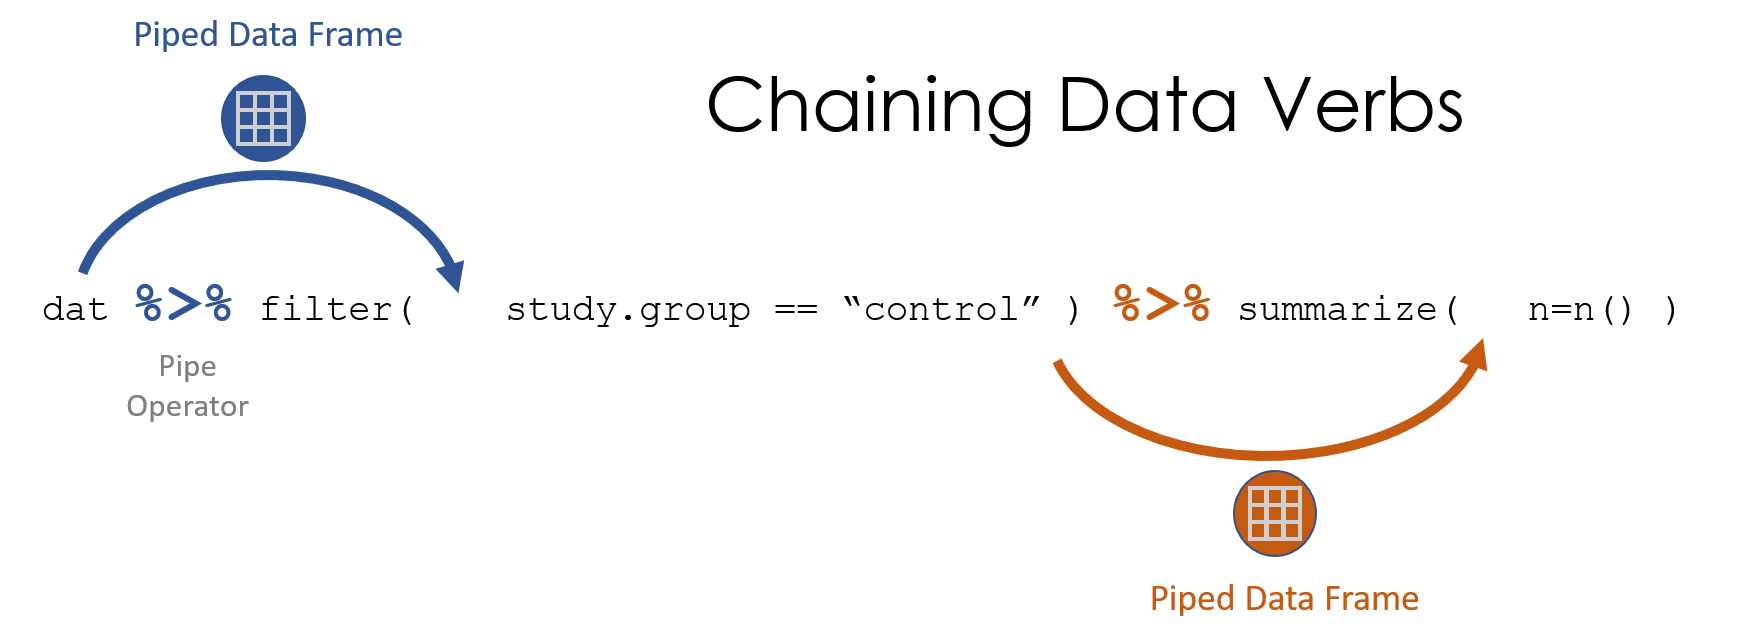
\includegraphics{chaining_data_verbs.png?raw=true}}{}}\label{section}}

\hypertarget{adding-a-pipe-in-rstudio}{%
\paragraph{Adding a Pipe in RStudio}\label{adding-a-pipe-in-rstudio}}

\hypertarget{you-can-easily-add-a-pipe-in-rstudio-using-the-keyboard-shortcut}{%
\paragraph{\texorpdfstring{You can easily add a pipe in RStudio using
the \textbf{keyboard
shortcut}:}{You can easily add a pipe in RStudio using the keyboard shortcut:}}\label{you-can-easily-add-a-pipe-in-rstudio-using-the-keyboard-shortcut}}

\#\#\#\#\textbf{Windows/Linux}: \texttt{Ctrl\ +\ Shift\ +\ M}
\#\#\#\#\textbf{Mac}: \texttt{Cmd\ +\ Shift\ +\ M}

\hypertarget{why-use-pipes}{%
\subsubsection{Why Use Pipes?}\label{why-use-pipes}}

\hypertarget{combining-pipes-with-functions-like-filter-from-the-dplyr-package-allows-you-to}{%
\subsubsection{\texorpdfstring{Combining pipes with functions like
\texttt{filter()} from the \texttt{dplyr} package allows you
to:}{Combining pipes with functions like filter() from the dplyr package allows you to:}}\label{combining-pipes-with-functions-like-filter-from-the-dplyr-package-allows-you-to}}

\hypertarget{simplify-your-code-by-chaining-multiple-functions-together.}{%
\paragraph{-Simplify your code by chaining multiple functions
together.}\label{simplify-your-code-by-chaining-multiple-functions-together.}}

\hypertarget{avoid-creating-intermediate-variables.}{%
\paragraph{-Avoid creating intermediate
variables.}\label{avoid-creating-intermediate-variables.}}

\hypertarget{improve-readability-and-make-complex-workflows-easier-to-follow.}{%
\paragraph{- Improve readability and make complex workflows easier to
follow.}\label{improve-readability-and-make-complex-workflows-easier-to-follow.}}

\hypertarget{example-filtering-data-with-pipes}{%
\paragraph{Example: Filtering Data with
Pipes}\label{example-filtering-data-with-pipes}}

\hypertarget{lets-use-pipes-to-filter-the-weather_data-dataset-to}{%
\paragraph{\texorpdfstring{Let's use pipes to filter the
\texttt{weather\_data} dataset
to:}{Let's use pipes to filter the weather\_data dataset to:}}\label{lets-use-pipes-to-filter-the-weather_data-dataset-to}}

\hypertarget{extract-cities-located-in-alaska.}{%
\paragraph{\texorpdfstring{1. Extract cities located in
\textbf{Alaska}.}{1. Extract cities located in Alaska.}}\label{extract-cities-located-in-alaska.}}

\hypertarget{keep-only-rows-with-precipitation-values-greater-than-1.}{%
\paragraph{\texorpdfstring{2. Keep only rows with precipitation values
greater than
\texttt{1}.}{2. Keep only rows with precipitation values greater than 1.}}\label{keep-only-rows-with-precipitation-values-greater-than-1.}}

\begin{Shaded}
\begin{Highlighting}[]
\KeywordTok{library}\NormalTok{(dplyr)}
\NormalTok{high_precipitation_cities_pipe <-}\StringTok{ }\NormalTok{weather_data }\OperatorTok
\StringTok{  }\KeywordTok{filter}\NormalTok{(Data.Precipitation }\OperatorTok{>}\StringTok{ }\DecValTok{5}\NormalTok{)}\OperatorTok
\StringTok{  }\KeywordTok{filter}\NormalTok{(Station.State}\OperatorTok{==}\StringTok{ "Alaska"}\NormalTok{)}
  

\CommentTok{# View the filtered data}
\KeywordTok{head}\NormalTok{(high_precipitation_cities_pipe)}
\end{Highlighting}
\end{Shaded}

\begin{verbatim}
##   Data.Precipitation  Date.Full Date.Month Date.Week.of Date.Year Station.City
## 1               7.30 2016-01-31          1           31      2016    Ketchikan
## 2               5.58 2016-02-07          2            7      2016    Ketchikan
## 3               6.42 2016-02-14          2           14      2016    Ketchikan
## 4              10.34 2016-02-28          2           28      2016    Ketchikan
## 5               5.76 2016-04-17          4           17      2016    Ketchikan
## 6               5.30 2016-05-08          5            8      2016      Yakutat
##   Station.Code Station.Location Station.State Data.Temperature.Avg.Temp
## 1          KTN    Ketchikan, AK        Alaska                        43
## 2          KTN    Ketchikan, AK        Alaska                        40
## 3          KTN    Ketchikan, AK        Alaska                        46
## 4          KTN    Ketchikan, AK        Alaska                        43
## 5          KTN    Ketchikan, AK        Alaska                        47
## 6          YAK      Yakutat, AK        Alaska                        43
##   Data.Temperature.Max.Temp Data.Temperature.Min.Temp Data.Wind.Direction
## 1                        47                        39                  19
## 2                        43                        36                  17
## 3                        49                        43                  14
## 4                        47                        39                  13
## 5                        51                        42                  12
## 6                        48                        38                  13
##   Data.Wind.Speed
## 1           10.46
## 2            9.00
## 3            9.81
## 4           12.08
## 5            8.64
## 6            4.58
\end{verbatim}

\begin{Shaded}
\begin{Highlighting}[]
\CommentTok{# Bar plot of precipitation by city}
\KeywordTok{ggplot}\NormalTok{(high_precipitation_cities_pipe, }\KeywordTok{aes}\NormalTok{(}\DataTypeTok{x =} \KeywordTok{reorder}\NormalTok{(Station.City, Data.Precipitation), }\DataTypeTok{y =}\NormalTok{ Data.Precipitation, }\DataTypeTok{fill =}\NormalTok{ Station.City)) }\OperatorTok{+}
\StringTok{  }\KeywordTok{geom_bar}\NormalTok{(}\DataTypeTok{stat =} \StringTok{"identity"}\NormalTok{) }\OperatorTok{+}
\StringTok{  }\KeywordTok{coord_flip}\NormalTok{() }\OperatorTok{+}\StringTok{  }\CommentTok{# Flip coordinates for readability}
\StringTok{  }\KeywordTok{ggtitle}\NormalTok{(}\StringTok{"Precipitation by City in Alaska (Data.Precipitation > 1)"}\NormalTok{) }\OperatorTok{+}
\StringTok{  }\KeywordTok{xlab}\NormalTok{(}\StringTok{"City"}\NormalTok{) }\OperatorTok{+}
\StringTok{  }\KeywordTok{ylab}\NormalTok{(}\StringTok{"Precipitation (inches)"}\NormalTok{) }\OperatorTok{+}
\StringTok{  }\KeywordTok{theme_minimal}\NormalTok{() }\OperatorTok{+}
\StringTok{  }\KeywordTok{theme}\NormalTok{(}\DataTypeTok{legend.position =} \StringTok{"none"}\NormalTok{)  }\CommentTok{# Remove legend for clarity}
\end{Highlighting}
\end{Shaded}

\includegraphics{Basics_R_files/figure-latex/unnamed-chunk-11-1.pdf}

\end{document}
